\exercise{Polygons and colours}

\paragraph{Explanation:}
I first defined several constants needed like the matrices required to draw the grid as well as the arrays for the pieces and in general all the colors.
The grid is drawn using the \mttext{fill} function, and the pieces are drawn with \mttext{patch} as using \mttext{fill} again would remove the grid.
Several helper functions are defined, e.g. \mttext{draw\_piece} which allows me to easily draw a single piece from an array of length 4.
One particular thing this function contains is a switch case to acurately do the rotations.
As suggested, I am using cell arrays to save the arrays used to show the pieces as well as their color.
Care has been put so that the figures do not overlap one another, however when exporting to png this does not seem to be fully consistent.

\paragraph{MATLAB Code:}

\begin{tiny}
    \verbatiminput{code/tetris.m}
\end{tiny}

\paragraph{Results:}

Figure 1 contains the result of the following example function call,
\begin{matlabcode}
    tetris([1,6,0,1;2,5,1,1;4,7,0,0;3,7,8,2;2,5,7,3;5,10,3,1;
            5,3,9,3;2,8,15,1;7,5,3,1;6,11,0,1;5,1,0,0;3,9,2,1]);
\end{matlabcode}

\begin{figure}[H]
    \centering
    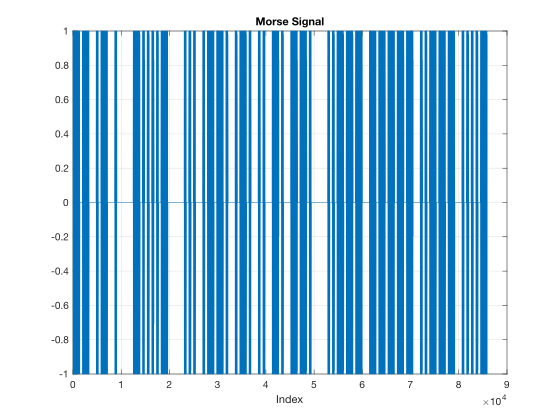
\includegraphics[width=12cm]{figures/ex1}
    \caption{Output of example call}
\end{figure}

\paragraph{Comments:}
The main difficulty I found was in defining the matrices to draw well the grid, I ended up looking at the MATLAB documentation for a similar functionality to the Python list comprehension.
The final result involved using cell arrays and the \mttext{cell2mat} function to convert back again to a matrix.
Then this resulting matrix is repeated using the \mttext{repmat} function to get the final matrix.
I tried my best to make the code easily modifyable (e.g. defining constants at the top) as well as modular by implementing several functions.
One can easily change the dimensions of the grid for example by changing the \mttext{HORIZONTAL\_SQUARES} and \mttext{VERTICAL\_SQUARES} constants.


\bigskip
\hrule


\exercise{Distorted plane}

\paragraph{Explanation:}
Here I really just followed the instructions, created mesh grids for the plane and sphere and then extract desired x, y, z coordinates from each.
For some reason for the Z displacement of the ball it took me a bit to realize my ball was centered at the origin instead of it being tangent to it.
Meaning I had to take the radius in consideration when displacing it.

\paragraph{MATLAB Code:}
\begin{tiny}
    \verbatiminput{code/plane.m}
\end{tiny}

\paragraph{Results:}
\begin{figure}[H]
    \centering
    \includegraphics[width=10cm]{figures/ex2}
\end{figure}

\paragraph{Comments:}
The trickiest part for me was playing around with the step sizes as well as colors to get the desired effect of the ball.
In the end I am pretty happy with the final result.

\bigskip
\hrule

\exercise{Sonine Polynomials}

\paragraph{Explanation:}
I started off by implementing a recursive function to calculate the sonine polynomials.
After reading the comments on the forum I switched to a classic bottom up DP approach using cell arrays to store all the intermediate polynomials.
Making the complexity of calculating a sonine polynomial linear with its degree.
I made the legend transparent to match with the example plot given using the \mttext{BackgroundAlpha} flag in the \mttext{legend} function.
I was also able to generalize with respect to $n$ and $\alpha$ which can be seen in the second figure.

\paragraph{MATLAB Code:}
\begin{tiny}
    \verbatiminput{code/sonine.m}
\end{tiny}

\paragraph{Results:}
\begin{verbatim}
S2:     0.5000   -3.5000    4.3750
S3:    -0.1667    2.2500   -7.8750    6.5625
S4:     0.0417   -0.9167    6.1875  -14.4375    9.0234
S5:    -0.0083    0.2708   -2.9792   13.4062  -23.4609   11.7305
\end{verbatim}

\begin{figure}[H]
    \centering
    \includegraphics[width=12cm]{figures/ex3}
    \caption{First 6 polynomials}
\end{figure}

\begin{figure}[H]
    \centering
    \includegraphics[width=12cm]{figures/ex3a}
    \caption{Showing the generalization}
\end{figure}

\paragraph{Comments:}
I looked for a way to pass by reference the DP variable so I could store intermediate polynomials between different calculations.
However the only was to accomplish this was to use global variables or return and keep the DP variable.
I ended going with a slightly less efficient approach where I am calculating (once) all polynomials up to n each time.
I thought this would make for cleaner code.

\bigskip
\